%!TEX root=../../Benutzerhandbuch.tex
\section{Schreiben eines Algorithmus}
Um die Software zu bedienen wird ein in \gls{F-Sharp} geschriebener Algorithmus ben�tigt. Dieser muss als \gls{DLL}-Datei zur Laufzeit in die Software eingebunden werden. Eine solche Datei wird mittels Microsoft Visual Studio erzeugt werden, damit die Software funktionieren soll. \\
Folgende Eigenschaften muss die Datei erf�llen:
\begin{itemize}
	\item Name der Methode: startCalculation
	\item �bergabeparameter 1: eine Liste aller historischen Daten 
	\item �bergabeparameter 2: eine Liste der Signale f�r die Entscheidungen (bei �bergabe ist diese Liste leer)
\end{itemize}
Mit dem R�ckgabewert der Methode wird nicht gearbeitet, sondern mit der vom Algorithmus verarbeiteten Signalliste.

\begin{lstlisting}[caption=Dateityp des 1. �bergabeparameters]{prices}
System.Collections.Generic.List<System.Tuple
<System.DateTime,decimal,decimal,decimal,decimal>>
\end{lstlisting}
\begin{lstlisting}[caption=Dateityp des 2. �bergabeparameters]{signals}
System.Collections.Generic.List<int>
\end{lstlisting}
Au�erdem muss sich der Algorithmus im Namespace  "`Algorithm"' und im Modul "`DecisionCalculator"' befinden.
\subsection{Erzeugen eines Algorithmus-Files}
�ffnen Sie Microsoft Visual Studio und erzeugen sie ein neues Projekt.\\
\begin{figure}[H]
\centering
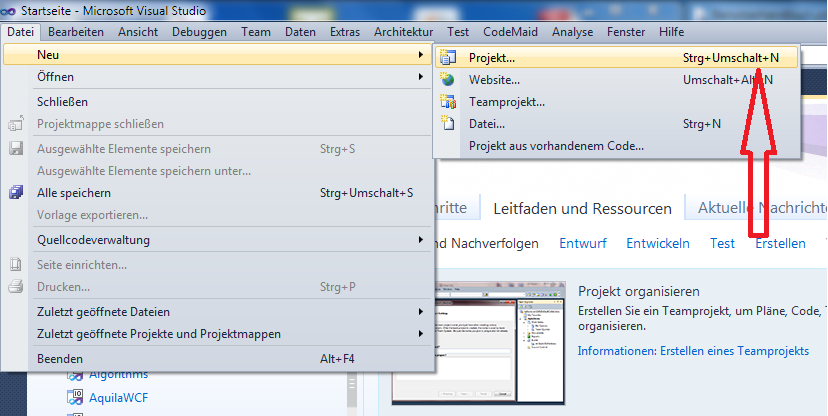
\includegraphics[width=1\textwidth]{images/newProject.png}
\caption{Erzeugen eines neuen Projekts}
\end{figure} 
\newpage
Erstellen Sie es als \gls{F-Sharp}-Bibliothek.
\begin{figure}[H]
\centering
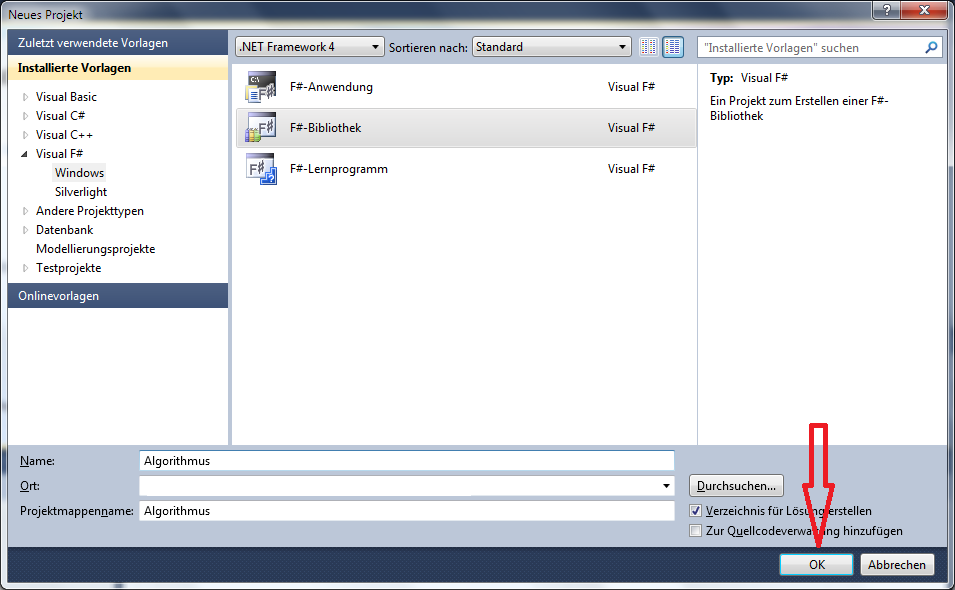
\includegraphics[width=1\textwidth]{images/createProject.png}
\caption{Erstellen Sie es als \gls{F-Sharp}-Bibliothek}
\end{figure}
Halten Sie sich an die, im Kapitel "`Schreiben eines Algorithmus"', genannten Richtlinien und implementieren die Methode startCalculation und kompilieren sie das Projekt.
\begin{figure}[H]
\centering
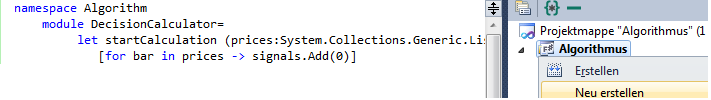
\includegraphics[width=1\textwidth]{images/makeFs.png}
\caption{Kompilieren des Projekts}
\end{figure}
\clearpage
\subsection{Entscheidungen}
Folgende Entscheidungen sind zul�ssig:
\begin{center}
\begin{tabular}{ |  p{1cm} | p{8cm} |}
\hline 
3 & starkes Kaufssignal \\ \hline
2 &   mittleres Kaufssignal \\ \hline
1 &  schwaches Kaufssignal\\ \hline
0 &  Alle Best�nde werden gekauft oder verkauft\\ \hline
-1 &  schwaches Verkaufssignal\\ \hline
-2 &  mittleres Verkaufssignal\\ \hline
-3 &  starkes Verkaufssignal\\ \hline
\end{tabular}
\end{center}
